Halide \cite{Ragan-Kelley:2013:HLC:2491956.2462176} is a domain-specific language designed for fast image processing and computational photography. Halide decouples the \emph{algorithm}, which defines \emph{what} values are computed, from the \emph{schedule}, which defines \emph{how} values are computed. Halide guarantees consistency -- an algorithm produces the same results no matter the schedule. Programmers are thus free to explore the space of schedules without introducing correctness bugs, and can vary the schedule per architecture without producing different results on different platforms.

Data-parallel operations, such as resizing an image, can be easily parallelized or vectorized in Halide. However, Halide does not support the same scheduling manipulations on reductions. To parallelize or vectorize a reduction, the programmer has to manually factor the reduction into multiple stages to expose new data parallelism. For example, instead of computing the histogram of an entire image, one might instead write an algorithm that computes the histogram of each row, and then adds those partial histograms. This need to rewrite the algorithm violates the core tenet of Halide: The algorithm should only specify \emph{what} is computed. It is the role of the schedule to specify \emph{how}. This manipulation of the \emph{algorithm} to parallelize reductions is bug-prone and hampers readability and portability. It is a language wart.

In this work, we present a new Halide scheduling primitive called \code{rfactor}, which moves this factoring of a reduction into the \emph{schedule}, while maintaining Halide's consistency guarantees. \code{rfactor} takes a Halide serial reduction (expressed with an unstructured Halide \emph{update} definition), and synthesizes the equivalent binary associative reduction operator and its identity. In some cases this synthesis problem is trivial. For example, given Halide code that sums a one-dimensional vector (Listing~\ref{lst:sum}), it is straightforward to deduce that the binary operator involved is addition, and its identity is zero. In other cases this synthesis problem is more challenging. Listing~\ref{lst:complex_magnitude} shows Halide code that finds the complex number with the greatest magnitude and its location within a two-dimensional array. It is not obvious what the equivalent associative binary operator is for this algorithm.

\begin{lstlisting}[float,
caption = {Halide sum reduction over a one-dimensional vector.}, label={lst:sum}]
Func out;
out() = 0;
RDom r(0, input.width());
out() = out() + input(r.x);
\end{lstlisting}


\begin{lstlisting}[float,
caption = {Halide reduction which finds the complex number with the greatest magnitude and its location in a two-dimensional array.}, label={lst:complex_magnitude}]
Func out;
out() = {0, 0, 0, 0};
RDom r(0, input.width(), 0, input.height());
Expr real = input(r.x, r.y)[0];
Expr imag = input(r.x, r.y)[1];
Expr mag = real * real + imag * imag;
Expr best_mag = out()[0] * out()[0] +
                out()[1] * out()[1];
Expr c = mag > best_mag;
out() = {select(c, real, out()[0]),
         select(c, imag, out()[1]),
         select(c, r.x, out()[2]),
         select(c, r.y, out()[3])};
\end{lstlisting}

During the compilation process, \code{rfactor} splits the original serial reduction into a pair of stages: The \emph{intermediate} stage computes partial results over slices of the domain of the reduction, and the \emph{merge} stage combines those partial results. The intermediate stage is now data parallel over the slices, which means that it can now be vectorized or parallelized using Halide's existing scheduling primitives.

Combined with other Halide scheduling primitives, such as \code{split}, \code{rfactor} allows Halide to represent a broad class of schedules for parallel and vectorized reductions. For example, rfactor can express several divide-and-conquer strategies for parallelizing and vectorizing the summation of a one-dimensional array (see Figure~\ref{fig:rfactor}).


\code{rfactor} further separates the \emph{algorithm} from its \emph{schedule} by making it possible to factor reductions using the schedule alone. In addition to the readability and portability benefits, this means that tools that automatically generate schedules \cite{Mullapudi:2016:ASH:2897824.2925952, Ragan-Kelley:2013:HLC:2491956.2462176} are now capable of parallelizing reductions, which was previously a task outside of their purview.

\begin{figure}
\centering
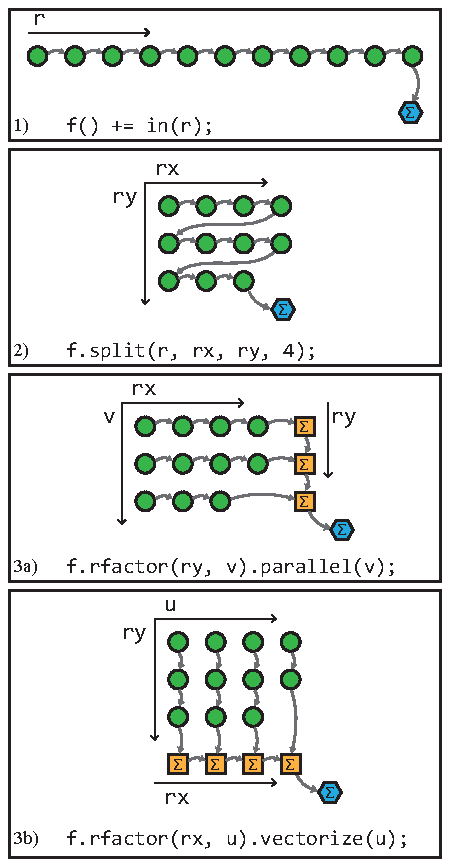
\includegraphics[width=\columnwidth]{rfactor}
\caption{%
\code{split} followed by \code{rfactor} used to vectorize or parallelize a one-dimensional summation. 1) A serial summation of 11 elements over a one-dimensional domain \code{r}. 2) The \code{split} scheduling directive reshapes the domain into a two-dimensional reduction. The reduction is still serial. 3a) The \code{rfactor} directive creates and returns a new (orange) \emph{intermediate} stage which computes partial results along each row. The intermediate stage is now data parallel over its outer loop, which is indexed with the new pure variable \code{v}. The merge stage (blue) retains only the serial loop over the reduction variable \code{ry}. We have \emph{reassociated} the summation. 3b) Alternatively, one can use rfactor to make the \emph{inner} loop data parallel. This can be used to vectorize reductions. The intermediate stage computes sums of whole vectors, data parallel across the vector lanes, and then the merge stage sums the lanes of the vector result. The strategies in 3a and 3b can be combined to both vectorize \emph{and} parallelize a summation.
}
\label{fig:rfactor}
\end{figure}

Our work makes the following contributions:
\begin{itemize}
  \item We introduce a new Halide scheduling primitive \code{rfactor} which factors a Halide reduction into pair of reductions: an \emph{intermediate} stage that computes partial results over slices of reduction domain and \emph{merge} stage that combines those partial results;
  \item We describe a method for automatically discovering an equivalent associative binary reduction operator and its identity from a serial reduction expressed as an imperative Halide \emph{update}.
  \item We implement a new stage in the Halide compiler that matches arbitrary reductions with a set of 17,905 fragments that are pre-generated using our synthesis method, and show that this enables the compiler to effectively transform a large set of reductions into their parallel equivalents.
\end{itemize}

The paper is structured as follows. Section~\ref{background} provides background on Halide and a discussion of related work. Section~\ref{assoc_red} presents the \code{rfactor} scheduling primitive and how it transforms Halide programs. Section~\ref{synthesize} describes the associative binary reduction operator synthesis technique. Section~\ref{evaluation} demonstrates that this technique does indeed produce the expected performance gains from vectorization and parallelization, and Section~\ref{conclusion} describes limitations and summarizes this work.


